\documentclass[]{report}
\usepackage[dvips]{graphicx}
\usepackage{amssymb}
\usepackage{placeins}
% Title Page
\title{NUbots Vision System Description}
\author{Shannon Fenn}

\begin{document}
\maketitle

\begin{abstract}
This document outlines the software architecture, major classes and expected configuration file formats of the NUbots Vision System as of March 2013.
\end{abstract}
\chapter{Software Architecture}
The vision system (see fig~\ref{fig:visionarchitecturefinal}) consists of a layered architecture consisting of an interfacial layer (to make the system more flexible and portable) and a processing layer. The processing layer itself follows the well known blackboard pattern from the AI community.

\begin{figure}[!htbp]
\centering
\vspace{2mm}
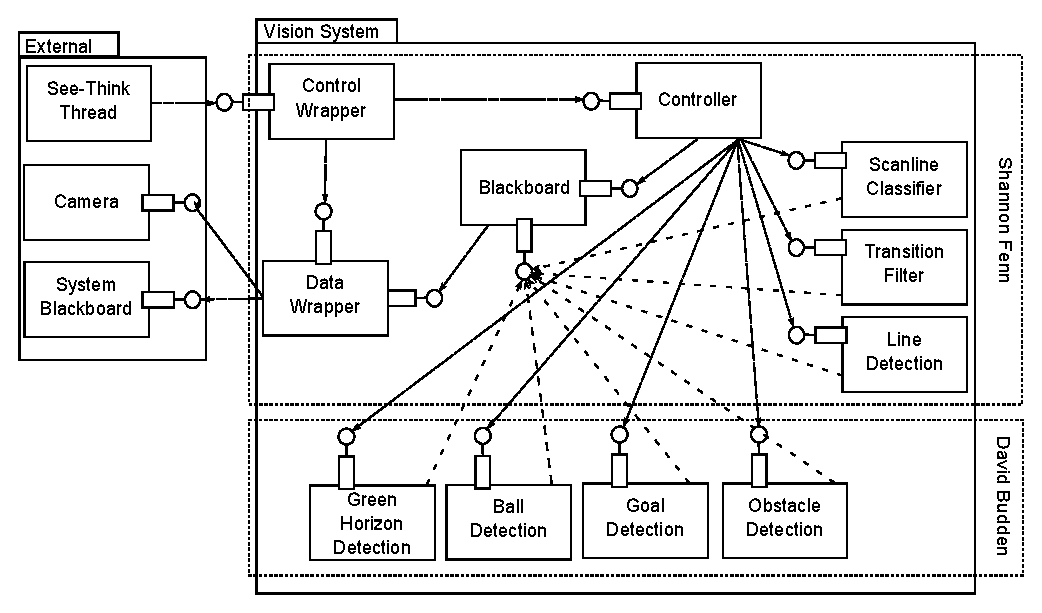
\includegraphics[scale=0.7,angle=0]{visionarchitecturefinal.eps}
\caption{\footnotesize Model of the Vision system framework - note the dual wrapper classes and the controller/blackboard classes. \normalsize}
\label{fig:visionarchitecturefinal}
\end{figure}

The \emph{control wrapper} exists as an external interface for invoking the vision system. This is key as vision is itself a subsystem. By designing this interface through a wrapper we trade a very slight decrease in efficiency (through a small number of redundant method calls) for a large increase in flexibility as the wrapper is the only module that need change for the system to be invoked in different ways (provided this change does not require the system's functional behaviour).

The \emph{data wrapper} exists as a way for the vision system to access the external data it needs (the image, kinematic data, sensor data etc). The same reasoning for modelling the control interface as a wrapper is applicable for the data interface. This approach also allows for data validity to be maintained. The data wrapper becomes responsible for maintaining the validity of data for each frame, i.e. it maintaining a copy of the relevant data accessed at the same time as the current frame if the external system cannot be trusted to do so. This insulates vision against poorly maintained external data structures. If the sensor data is updated by the locomotion system whilst the vision system is midway through analysing a frame the data wrapper still has a local copy. This decouples the data responsibilities of the various systems and ensures vision is as robust as possible to change.

Having these interfaces as wrappers has one extra advantage: rapid testing. Either wrapper can be replaced by a stub providing either dummy data in the case of the data wrapper or invoking the system with extra debugging information or only after user triggering. This has allowed for the system to be quickly integrated into a desktop application interfacing with a standalone webcam, without kinematic or sensor data, into the NUbots NUView system, which reads the appropriate data from log files or network streams and also onto the RaspberryPi platform.

The centralised \emph{blackboard} was implemented follows the singleton pattern. This is for two reasons: firstly the blackboard is a single object throughout the system and it should not be possible for multiple to be instantiated, secondly it allows for simple global access in the form of a static access method. The blackboard forms a central repository of current state information, each processing stage in the system requests the input it needs from the blackboard and posts results back. This increases the complexity of the system somewhat by requiring correct process order to be maintained by a controller, but allows for rapid reordering of independent stages and implementation of new stages.

The \emph{controller} at present simply calls processing stages in order with stages optionally ignored (for example ball or landmark detection). This allows for current state knowledge to increase the efficiency of the vision, for example when the localisation system has a high certainty of the present location but a low certainty of the relative ball location it does not need landmark information readily while it does need behaviour and vision to find and identify the ball quickly. By suppressing landmark detection the vision system can reduce its processing time freeing up resources for other processes.

\chapter{Major Classes and Directories}
\section{Control and Data Wrapper (singletons)}
The Control Wrapper class is redefined in several files, and in each provides whichever interface the external system requires, in most cases this is simply a per-frame runFrame() command, or a continuous run() command, each has a corresponding data wrapper described below.

The Data Wrapper class is redefined in several files and in each it provides the same minimal interface but a different internal implementation. This class is responsible for communication between the main vision system and whatever external system or interface is using it, be that NUView, the main robot framework, or the stand-alone offline development framework (the "Vision" Qt project). It has a number of publish, debugPublish (useful for providing intermediary data to an external system that is not part of the formal output), and access methods.

Any new implementation of this class should insulate the internal system from external faults (by copying data structures etc. where necessary), and is responsible for reformatting the Vision system outputs to fit external requirements. In order for the internal system to be able to use the appropriate wrapper an inclusion selection header DataWrapperCurrent.h is included. This header uses previously defined precompiler constants to determine which header to pass forward. When building projects with new wrappers, or which reuse old wrappers simply look at this file to decide which precompiler constants need to be defined.

Currently there are 4 versions of the wrappers, indicated by the following suffices in the file names:
\begin{description}
\item[PC] This is the wrapper for the standalone version, it provides runtime selection between interfacing with a USB webcam or reading from selected file streams and displays output to a graphical interface using the open source Qt framework.
\item[Darwin] This is the wrapper for the main framework, it interfaces with the central Blackboard and publishes detections to the external FieldObjects container.
\item[NUView] This is the wrapper for the NUView debug system, with NUView's internal network and stream readers and publishes results to the NUView FieldObjects container - NUView is responsible for displaying these.
\item[RPi] This an unfinished wrapper for the RaspberryPi, it interfaces with a USB webcam and indicates detections by toggling mapped GPIO pins high or low.
\end{description}

\section{VisionController}
This class maintains the instances of the various modules as well as the internal Blackboard, this class provides a single runFrame() command which requests the internal Blackboard to refresh its internal members via the current Data Wrapper instance, then calls each of the detection modules in the appropriate order and then requests that the internal Blackboard publish whichever results it via the same Data Wrapper.

\section{VisionBlackboard (singleton)}
Contains the main data held by the system for the duration of a frame, including the initial image and transformation information, and the results from all modules. All data on the blackboard is purged and replaced frame-to-frame, if new structures are added to the blackboard ensure they are correctly maintained in this way in the update() method. The blackboard updates itself (upon instruction by the controller) at the start of each frame from the data wrapper, and publishes the system's final results (again when instructed by the controller) through the same wrapper. Note that as each field object is published in a different way the actual process of publishing involves passing a pointer to the external field objects container through to each resulting visual object and allowing it to insert itself as an ambiguous object or modify the static object it represents based on its own internal data.

\section{BasicVisionTypes}
This is not a class but rather a header and source for several global enumerated type definitions and mappings to and from integral and string representations. This also includes some typedef statements for commonly used templated types (in order to increase readability). When changing any of these enumeration definitions in the header be sure to reflect these changes in the private mapping classes defined in the source, the mapping methods themselves use these classes (inherited from std::map) and thus do not need to be modified.

\section{VisionTypes}
\subsection{Quad}
This represents a convex quadrilateral in the image plane and forms the basis for goal and obstacle objects. It is a simple type consisting of four corner points along with accessor methods to easily obtain important information such as the bottom-centre position, centre position, mean width, mean height, area and determine intersections.
\subsection{GreenHorizon}
This type represents the field border and internally consists of a set of points provided by the green horizon detection module as well as a list of interpolated points (trading spatial efficiency for temporal efficiency by pre-calculating once rather than several times). This type also allows the retrieval of a single y-value or a series of interpolated points with any given pixel spacing and a function to check if a given point is below the horizon (useful for filtering). Linear interpolation is used for efficiency reasons though the implementation is such that any other method could reasonably be used with little modification by simply replacing the interpolation function.
\subsection{ColourSegment}
This type is used to represent a continuous run of pixels with the same colour classification. The type internally consists of a colour and two end points, the length and centre-point of the segment are pre-calculated and maintained as well for efficiency since it they are queried multiple times per frame. This type allows the obvious accessors as well as having input and output stream operators (for file IO) and a method to allow the joining of an adjacent segments (used for replacement rules discussed later).
\subsection{SegmentedRegion}
This type exists to maintain all of the classified segments in a logical structure. It is a list of lists of segments as well as an alignment. Within the current implementation there are only ever two - one for the vertical and one for the horizontal segments, however it is not restricted to that. It is this data-type that the initial filters operate on to produce the information that the object classifiers rely on.
\subsection{ColourRule}
This represents an abstract rule used by various colour filters (replacement and transition rules). It consists of three lists (before, middle and after) of colour-classes each with an associated numeric range. The standard accessor methods exist as well as a function for matching the rule to a triplet of segments and stream operators (important since the rules are meant to be read in from file in order to make the system highly configurable without requiring recompilation).
\subsection{ColourReplacementRule}
This represents a rule used by the replacement filter. It consists of a name, an enumerated replacement method (for now - before, after and split) and a before as well as the inherited types and methods from the more abstract Rule type.
\subsection{ColourTransitionRule}
This is a rule used by the transition detection filter described later, and is similar to the ColourReplacementRule but instead of a name and replacement method the transition rule has a object-class that it belongs to (presently post, ball or line).
\subsection{GroundPoint}
This class is an attempt to unify multiple coordinate representations for points that are known to be on the ground. It consist of 2D vectors representing the points Cartesian coordinates in the image plane, radial coordinates relative to the camera vector and Cartesian coordinates relative to the robot in the field plane as well as a 3D vector representing its radial coordinates in the world space.
\subsection{Histogram1D}
This describes a uni dimensional histogram, which is used for the histogramming goal detection method, but which could be used for other purposes.
\subsection{Interfaces}
This includes three pure abstract classes which serve as interfaces:
\begin{description}
\item[Publishable] The methods which must be provided for an object to be publishable to the external field objects container within the main robocup framework.
\item[Optimisable] The methods which must be provided for a type to be used in the optimisation framework (basically deprecated).
\item[RANSACModel] The methods which should be provided for a type to be a Model for the RANSAC implementation, unfortunately there is no way for templating within c++ to enforce subtyping so this is only a recommended not a required interface.
\end{description}
\subsection{RANSACTypes}
This directory includes the model types that have been defined so far for RANSAC instantiations within the system.
\subsection{VisionFieldObject}
This class and its children describe publishable (except in the case of lines) objects and inherits from some custom interfaces. This class contains the common minimum information and interface required by the system and any external systems to describe the visual and spatial properties of objects in the field of play. Each child class obviously includes specialised information and defines how it is to be published to an external field object, represented in and transformed between the camera plane and field space and compared for optimisation purposes. These child classes are currently: Ball, Goal, Obstacle, FieldLine, CornerPoint and CentreCircle.

\section{General Algorithms}
This subdirectory is intended to include any algorithms that may be generically applied within the vision system, but currently only contains a generic templated implementation of the RANSAC algorithm. This  implementation requires a Model class and a DataPoint type for which the Model must implement at a minimum:
\begin{description}
\item[int minPointsForFit()] Returns the minimum number of data points required to uniquely fit a model.
\item[bool regenerate(vector<DataPoint>)] Attempts to regenerate the model, fitting it to the provided data points, returns success/failure.
\item[double calculateError(DataPoint)] Returns a decimal representation of how much the provided point disagrees with the model (in most cases a distance of a point in $\mathbb{R}^n$ from a geometric model).
\end{description}
This is implemented as a series of functions within a namespace rather than a class (much like BasicVisionTypes). This means that using RANSAC involves simply calling one of two static functions:
\begin{description}
\item[findMultipleModels] returns multiple pairs of fit models and corresponding consensus sets.
\item[findModel] returns an indication of success explicity and via reference variables provides a fit model, consensus dataset, non consensus data set and mean error (variance).
\end{description}

Both require several parameters:
\begin{description}
\item[e] The error bound within which a datapoint will be considered to ``agree'' with the model.
\item[n] The minimum number of consensus points to consider a model successfully found, if this is less than minPointsToFit() or larger than the number of provided datapoints then obviously no models will be found.
\item[k] The number of random models to be tested before the best is kept.
\item[method] An element of an enumerated type which lists the methods for evaluating the fitness of models relatively. Currently this consists of the self explanatory LargestConsensus and BestFittingConsensus.
\end{description}
The findMultipleModels function also requires a numeric upper bound for the number of models which can be found. More information can be kept by manually calling findModel however findMultipleModels will automatically manage the repeated calls and point set manipulation required for multiple attempts.

\section{Modules}
This includes the detection modules used by the system for finding the ball, goalposts, fieldlines, corners, the centre circle and obstacles. The actual algorithms are complicated and described within Shannon Fenn and David Budden's final year reports and as such not described here (yet).

\section{VisionTools}
This includes:
\begin{description}
\item[PCCamera] A class which allows retrieval of an image from a USB webcam for the offline testing system.
\item[ClassificationColours] A class which describes the colours which can be classified within the lookuptable.
\item[LookupTable] A class which allows conversion between a 3D colour space vector (pixel) and a class label via a 128x128x128 char array.
\item[Transformer] A class which allows transformation between the various spaces used by the vision system, utilising kinematics data collected at the start of the frame as well as the known pixel dimensions and field of view of the camera.
\end{description}

\chapter{Configuration Files}

\section{Rules}
The Vision system reads the rules it uses for noise filtering and transition detection from file. 

For replacement rules (those used to filter classification noise) the expected layout is a series of newline separated rules of the form:
\begin{verbatim}
name:
before: (min_b, max_b) [colour0, colour1]   //comment
middle: (min_m , max_m) [colour2]           //comment
after: (min_a, max_a) [colour3]             //comment
replacement: method                         //comment
\end{verbatim}

Where the min and max values are integer pixel numbers (relative values which expresses a fraction of the image width or height were toyed with, but proved difficult to modify by hand) and \emph{method} is one of ``before'', ``after'' or ``split''. This method describes which colour the middle segment will be replaced with. Within each pair of square braces an unbounded comma separated list of colours to which rule could possibly be matched is given.  An example, used to filter shot noise in the field, is given below:
\begin{verbatim}
fieldnoise_v_small:
before: (3, 320) [green]         //3 pix min
middle: (0 , 1) [unclassified]   //1 pix max
after: (3, 320) [green]          //3 pix min
replacement: before              //before, after, split
\end{verbatim}

Within the ``Rules'' directory of the configuration directory there must be two of these files, one which is used on vertical segments, and one on horizontal. This could be changed by adding an extra option to the format which specifies the direction (vertical, horizontal or both) to which the rule applies and only reading in rules from a single file.

For transition rules (those used to filter potential field object points) the expected layout is a series of newline separated rules of the form:

\begin{verbatim}
COLOUR_CLASS:
before: (min_b, max_b) [colour0, colour1]   //comment
middle: (min_m , max_m) [unclassified]      //comment
after: (min_a, max_a) [green]               //comment
\end{verbatim}

The only difference in format between replacement and transition rules is that instead of a name, transition rules are labelled by a COLOUR\_CLASS which must match one of the elements of the enumerated type with the same name in BasicVisionTypes, and that transition rules lack a replacement method field.

The filenames expected are \emph{ReplacementRules\_h.txt}, \emph{ReplacementRules\_v.txt}, \emph{TransitionRules\_h.txt} and \emph{TransitionRules\_v.txt} and are loaded within the constructor of the SegmentFilter module. In actuality this was an inflexible design choice and at some point in the future these rules should be made to reside on the blackboard and be loaded from the wrapper at each frame (this would allow automated testing or learning of the rules which at present have not been modified much since they were first created). Figure~\ref{fig:rep_rules_vs_gaussian} shows why we use replacement rules rather than a Gaussian or similar blurring method.

\begin{figure}[!htbp]
\centering
\vspace{2mm}
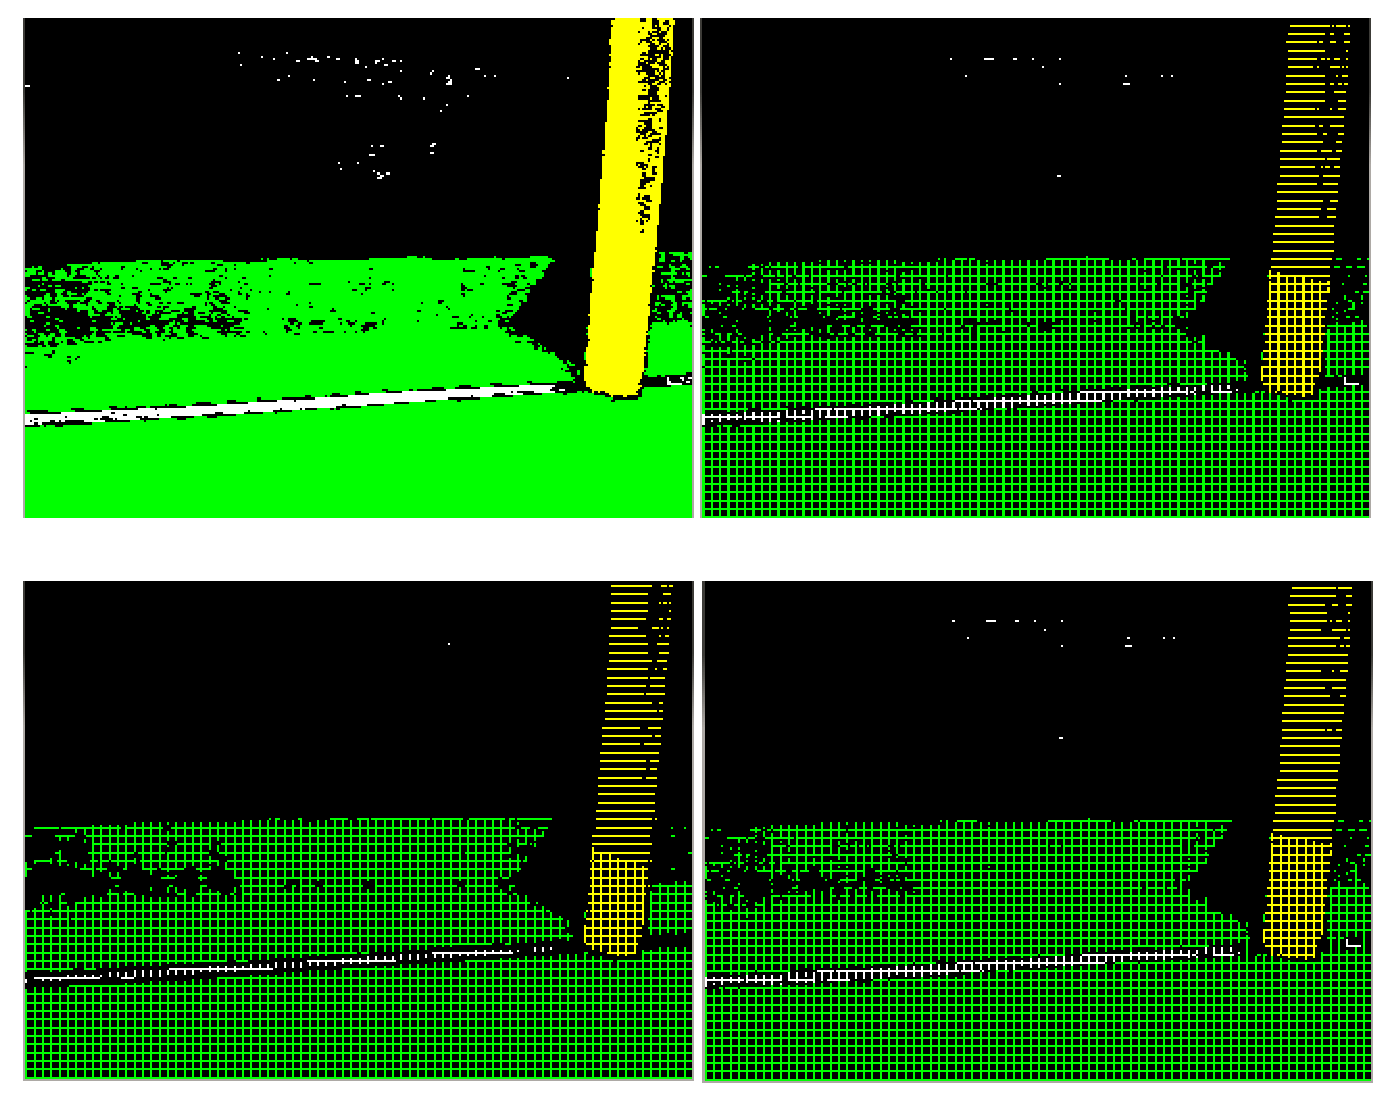
\includegraphics[scale=0.45,angle=0]{rep_rules_vs_gaussian.eps}
\caption{\footnotesize LUT classified image (top-left). Segments before filtering (top-right). Segments from a blurred image (bottom-left). Segments after replacement rule filtering (bottom-right). \normalsize}
\label{fig:rep_rules_vs_gaussian}
\end{figure}
\FloatBarrier

\section{VisionOptions.cfg}
VisionOptions.cfg and its relating class ``VisionConstants'' are poorly maintained and should be replaced with new configuration system. Nonetheless this file is currently expected to exist within the configuration directory of the robot, or within robocup/Config/NUView, when using NUView, or manually selected by the user when using the off-line Vision program. It is a newline separated list of entries in the form ``CONSTANT\_NAME: value'' where CONSTANT\_NAME matches the name of a constants within VisionConstants and value is the boolean (0/1, not true/false), integer or decimal value being given or is a string that indicates an enumerated option. An example subset is given below, note that as much horizontal or vertical whitespace as desired can be used to help readability:

\begin{verbatim}
BALL_DISTANCE_METHOD:                   D2P
GOAL_DISTANCE_METHOD:                   D2P

BALL_EDGE_THRESHOLD:                    15
BALL_ORANGE_TOLERANCE:                  25
BALL_MIN_PERCENT_ORANGE:		0.2
MIN_GOAL_SEPARATION:            40

GOAL_WIDTH:             10
GOAL_HEIGHT_INTERNAL:   80
DISTANCE_BETWEEN_POSTS: 150
BALL_WIDTH:             6.5
CENTRE_CIRCLE_RADIUS:   60

LINE_METHOD:	                RANSAC
RANSAC_MAX_ANGLE_DIFF_TO_MERGE: 0.1
RANSAC_MAX_DISTANCE_TO_MERGE:   10
\end{verbatim}

\end{document}
